\documentclass[11pt]{report}
\usepackage[a4paper]{geometry}
\usepackage[myheadings]{fullpage}
\usepackage{fancyhdr}
\usepackage{lastpage}
\usepackage{graphicx, wrapfig, subcaption, setspace, booktabs}
\usepackage[T1]{fontenc}
\usepackage[font=small, labelfont=bf]{caption}
\usepackage[protrusion=true, expansion=true]{microtype}
\usepackage{sectsty}
\usepackage{url, lipsum}
\usepackage{mathptmx}
\usepackage[utf8]{inputenc}
\usepackage[francais]{babel}
\pagestyle{plain}

\newcommand{\HRule}[1]{\rule{\linewidth}{#1}}
\onehalfspacing
\setcounter{tocdepth}{5}
\setcounter{secnumdepth}{5}

\renewcommand{\thesection}{\arabic{section}}

%-------------------------------------------------------------------------------
% TITLE PAGE
%-------------------------------------------------------------------------------

\begin{document}

\title
{
	\Large{Projet de communication transdisciplinaire}
	\HRule{2pt} \\ [0.5cm]
	\LARGE \textbf{\uppercase{Bacchanight}}
	\HRule{2pt} \\ [0.5cm]
	\normalsize \today
}

\date{}

\author
{
	\LARGE{Université de Bordeaux} \\
	\\
	Guillaume CHARLET \\
    Kenji FONTAINE \\
    Gauthier LAMARQUE \\
}

\maketitle

%-------------------------------------------------------------------------------
% Présentation du projet
%-------------------------------------------------------------------------------

\renewcommand{\thesection}{\arabic{section}}

\section{Présentation du projet}

La Baccha-night, du mot « bacchanales », fêtes mythologiques en l’honneur du
dieu du vin Bacchus, est un évènement nocturne étudiant proposé par le musée
des Beaux-Arts de Bordeaux le mardi 21 mars 2017.
Le but de ce projet est d'élaborer un outil permettant de mieux renseigner
les internautes sur la soirée (programme, accès, réseaux sociaux, etc.). \\
Ce projet a été mené sur l'ensemble de l'année scolaire 2016/2017. Les membres
composants l'équipe a pu changer au cours de l'année. De ce fait, le rapport est
divisé en deux parties, une pour chaque semestre.

\section{Premier semestre}

L'équipe est initialement composé de :
\begin{itemize}
 	\item Julien COUVY
    \item Kenji FONTAINE
    \item Gauthier LAMARQUE
    \item Enzo PERUZZETTO
	\item Guillaume CHARLET (qui nous rejoindra un peu plus tard)
\end{itemize}

\subsection{Déroulement}

Pour les premières séances, notre priorité était d'avoir une idée claire
de ce que nous devions faire. Nous avons alors commencé par nous renseigner sur
ce qu'était la Bacchanight. Après une séance de recherche et de mise en commun,
nous avons vu, qu'en effet les informations étaient difficiles à trouver.
\par
Nous nous sommes alors demandé quelle forme pourrait prendre un outil numérique
permettant une bonne transmission des informations. Finalement, nous avons décidé
que faire un site web dédié à la soirée serait une bonne solution. \\
Ensuite, nous avons regardé différents sites présentant des événements similaires
à la Bacchanight afin d'avoir une meilleure idée de ce qui était attendu d'un
tel site. Suite à cette recherche, le modèle "Page unique" ou "One Page" a été
retenu de par sa simplicité et son efficacité. \\
C'est à ce moment que \textit{Guillaume Charlet} a rejoint notre équipe.
\par
Le prochain objectif pour notre groupe était alors de mettre sur papier,
la forme qu'allait prendre notre page. Barre de navigation, boutons,
système utilisateurs, système permettant de commenter, photos, vidéos, carousel... \\
Le prototype ainsi obtenu est disponible en annexe.

\subsection{Choix des technologies}

Afin de faciliter le déploiment et la mise en ligne de notre travail, utiliser la
même technologie que le site actuel du Musée des Beaux Arts est le plus simple.
Nous avons ainsi décider d'utiliser le même système de gestion du contenu
\textbf{Drupal 7}. \\
Cela ajoute une nouvelle difficulté au projet: Notre produit doit être facilement
exportable, afin que la mise en ligne de la page web soit réalisable.

Le site doit permettre l'accès aux informations suivantes :
\begin{itemize}
	\item Description de la soirée,
	\item Date et lieu,
	\item Programme de la soirée,
	\item Photos de l'événement,
	\item Remerciements et Partenaires,
	\item Contact, lien vers les réseaux sociaux du Musée des Beaux Arts.
\end{itemize}

\vspace{0.5cm}

\subsection{Champs modifiables}

\subsubsection{Couleur principale}

La couleur principale est décrite par un champ texte d'une longueur maximale de
7 caractères. La couleur est exprimée en hexadécimal de la façon suivante :
\textbf{\#000000} à \textbf{\#FFFFFF}. \\
Cette couleur est utilisée pour les éléments suivants de la page :
\begin{itemize}
	\item La mise en valeur d'un élément dans la barre de navigation.
	\item Le bouton "Découvrez Bacchanight!" inclus dans l'image d'en-tête.
	\item L'écriture des balises \textbf{[G]} et \textbf{[M]} indiquant le lieu d'un événement dans le programme.
	\item Le bouton "Envoyer" dans la section \textbf{Contact}.
	\item L'écriture des catégories d'informations en bas de page.
	\item La partie basse de l'effet dégradé en bas de page.
\end{itemize}

\subsubsection{Couleur niveau de gris}

TODO.

\subsubsection{Image fond}

L'image de fond est utilisé comme image d'en-tête. Elle est également utilisé
pour les bannières \textbf{Programme}, \textbf{Galerie}, \textbf{Contact} et
\textbf{Partenaires}. L'effet bichromie est obtenu automatiquement ? L'effet
bichromie n'est pas automatique, vous devez l'appliquer à la main. ?
Ce champ image est stocké et est modifiable via Drupal. \\
Les extensions acceptées sont les suivantes : \textbf{png, gif, jpg, jpeg}.

\subsubsection{Image description}

Cette image est affichée à gauche du texte de description. Lorsqu'un utilisateur
passe son curseur sur l'image, celle-ci passe en couleur. Cet effet est automatique.
Ce champ image est stocké et est modifiable via Drupal. \\
Les extensions acceptées sont les suivantes : \textbf{png, gif, jpg, jpeg}.

\subsubsection{Description}

La description de la soirée est un champ texte stocké par Drupal. Il est
modifiable par une personne ayant les droits d'administration sur Drupal.
Seulement quelques balises HTML sont autorisées, les autres sont ignorées.
(à compléter)...

\subsubsection{Programme}

Le programme est généré à partir d'un fichier texte que l'administrateur
uploadera? à partir du pannel d'administration de Drupal. \\
Le fichier devra être rédigé de la façon suivante :
\begin{verbatim}
	l.1 Horaires de l'événement 1
	l.2 Titre de l'événement 1
	l.3 Description de l'événement 1
	l.4 Emplacement de l'événement 1 (G ou M)
	l.5 (Laisser une ligne vide)
	l.6 Horaires de l'événement 2
	l.7 Titre de l'événement 2
	l.8 etc...
\end{verbatim}

\subsubsection{Image Programme}

Cette image est affichée à droite de la section \textbf{Programme}. De même que
pour \textbf{l'Image Description}, l'effet couleur est automatique.
Ce champ image est stocké et est modifiable via Drupal.

\subsubsection{En continu}

La section \textbf{En continu} est géré de la même façon que le \textbf{Programme}.
Les fichiers texte générant ces deux sections sont rédigés de la même façon.
Un fichier correspond à une seule section du Programme. Il faut donc deux fichiers
texte, un pour le "Programme" et un pour le "En continu".

\subsubsection{Galeries}

Ces images seront affichées dans la section \textbf{Galeries} du site. TODO.

\subsubsection{Captcha Key}

TODO.

\subsubsection{Texte partenaire}

TODO.

\subsubsection{Image partenaire}

TODO.

\subsubsection{Date et heure}

La description de la soirée est un champ texte stocké par Drupal. Il est
modifiable par une personne ayant les droits d'administration sur Drupal.
L'utilisateur n'a aucun contrôle sur la forme prise par la date, mise à part la
façon dont il insère la date. \\
\textbf{exemple :} DD/MM/YYYY ou Day DD Month YYYY. \\

L'heure est un autre champ texte, stocké et modifiable de la même façon que la
date.
L'utilisateur n'a, là aussi, aucun contrôle sur la forme au-delà de la façon
dont l'heure est insérée dans le champ texte.
\textbf{exemple :} HH : MM - HH : MM \\

\subsubsection{Contact téléphone}

TODO.

\subsubsection{Contact mail}

TODO.

\subsubsection{Réseaux sociaux}

TODO.

\subsubsection{Copyright}

TODO.

%-------------------------------------------------------------------------------
% Besoins non fonctionnels
%-------------------------------------------------------------------------------

\subsection*{Hébergement}
Prise de contact avec la Mairie de Bordeaux, actuellement chargée de
l'hébergement du site du Musée des Beaux-Arts.

\subsection*{Déploiement}
Création de la page en utilisant le système de gestion de contenu Drupal
(version 7) déjà présent sur le site du Musée des Beaux-Arts.
Un manuel permettant à une personne ayant de l'expérience avec Drupal
d'intégrer le site au site actuel du musée devra être fourni.

%-------------------------------------------------------------------------------
% Besoins non fonctionnels
%-------------------------------------------------------------------------------

\section{Besoins non fonctionnels}

\subsection*{Charte graphique}

En ce qui concerne la charte graphique, le musée des Beaux Arts de Bordeaux nous a transmis un document (disponible en annexe) regroupant tous les éléments graphiques (images, polices, logos, etc.) que nous avons intégrés au site.

Le site est sous un format One Page. Un site One Page est un site constitué
d'une seule et même page sur laquelle l'ensemble des informations du site web
est disponible en scrollant (ou à l'aide d'une barre de navigation).

\subsection*{Accessibilité}

Le site doit être accessible à partir des navigateurs suivants (toutes plateformes confondues):
%% Ajouter les numéros de versions.
\begin{center}
	\begin{tabular}{|l | r|}
		\hline
		Navigateurs & Parts de marché \\
		\hline
		\hline
		Google Chrome 54+ & 51\% \\
		\hline
		Mozilla Firefox 51.0+ & 7,4\% \\
		\hline
		Safari (Apple) 10.0+ & 18,3\% \\
		\hline
		Microsoft Edge / IE 11.0 & 10,8\% \\
		\hline
	\end{tabular}
\end{center}
Ces navigateurs ont été sélectionnés à partir de leur pourcentage de parts de marché (toutes supérieures à 5\%). Ce pourcentage est une moyenne des pourcentages recueillis sur les sites suivants:
\begin{itemize}
	\item StatCounter
	\item Net MarketShare
	\item W3Counter
	\item Akamai
\end{itemize}

\subsection*{Responsive}
Puisque le site doit être accessible depuis plusieurs plateformes, le site doit s'adapter à la taille de l'écran.

\subsection*{Léger}
Le site doit se charger en moins de X secondes, en utilisant une connection à
X ko/s. (à tester)

%-------------------------------------------------------------------------------
% Retro planning
%-------------------------------------------------------------------------------

\section{Retro planning}

\begin{itemize}
	\item Version statique pour avant le 21 Mars. (priorité haute)
	\item Version pérenne pour la fin du semestre. (mi-Avril, à confirmer)
\end{itemize}

%-------------------------------------------------------------------------------
% Maquette
%-------------------------------------------------------------------------------

\newpage

\section{Annexe : Maquette}

\vspace{0.4cm}
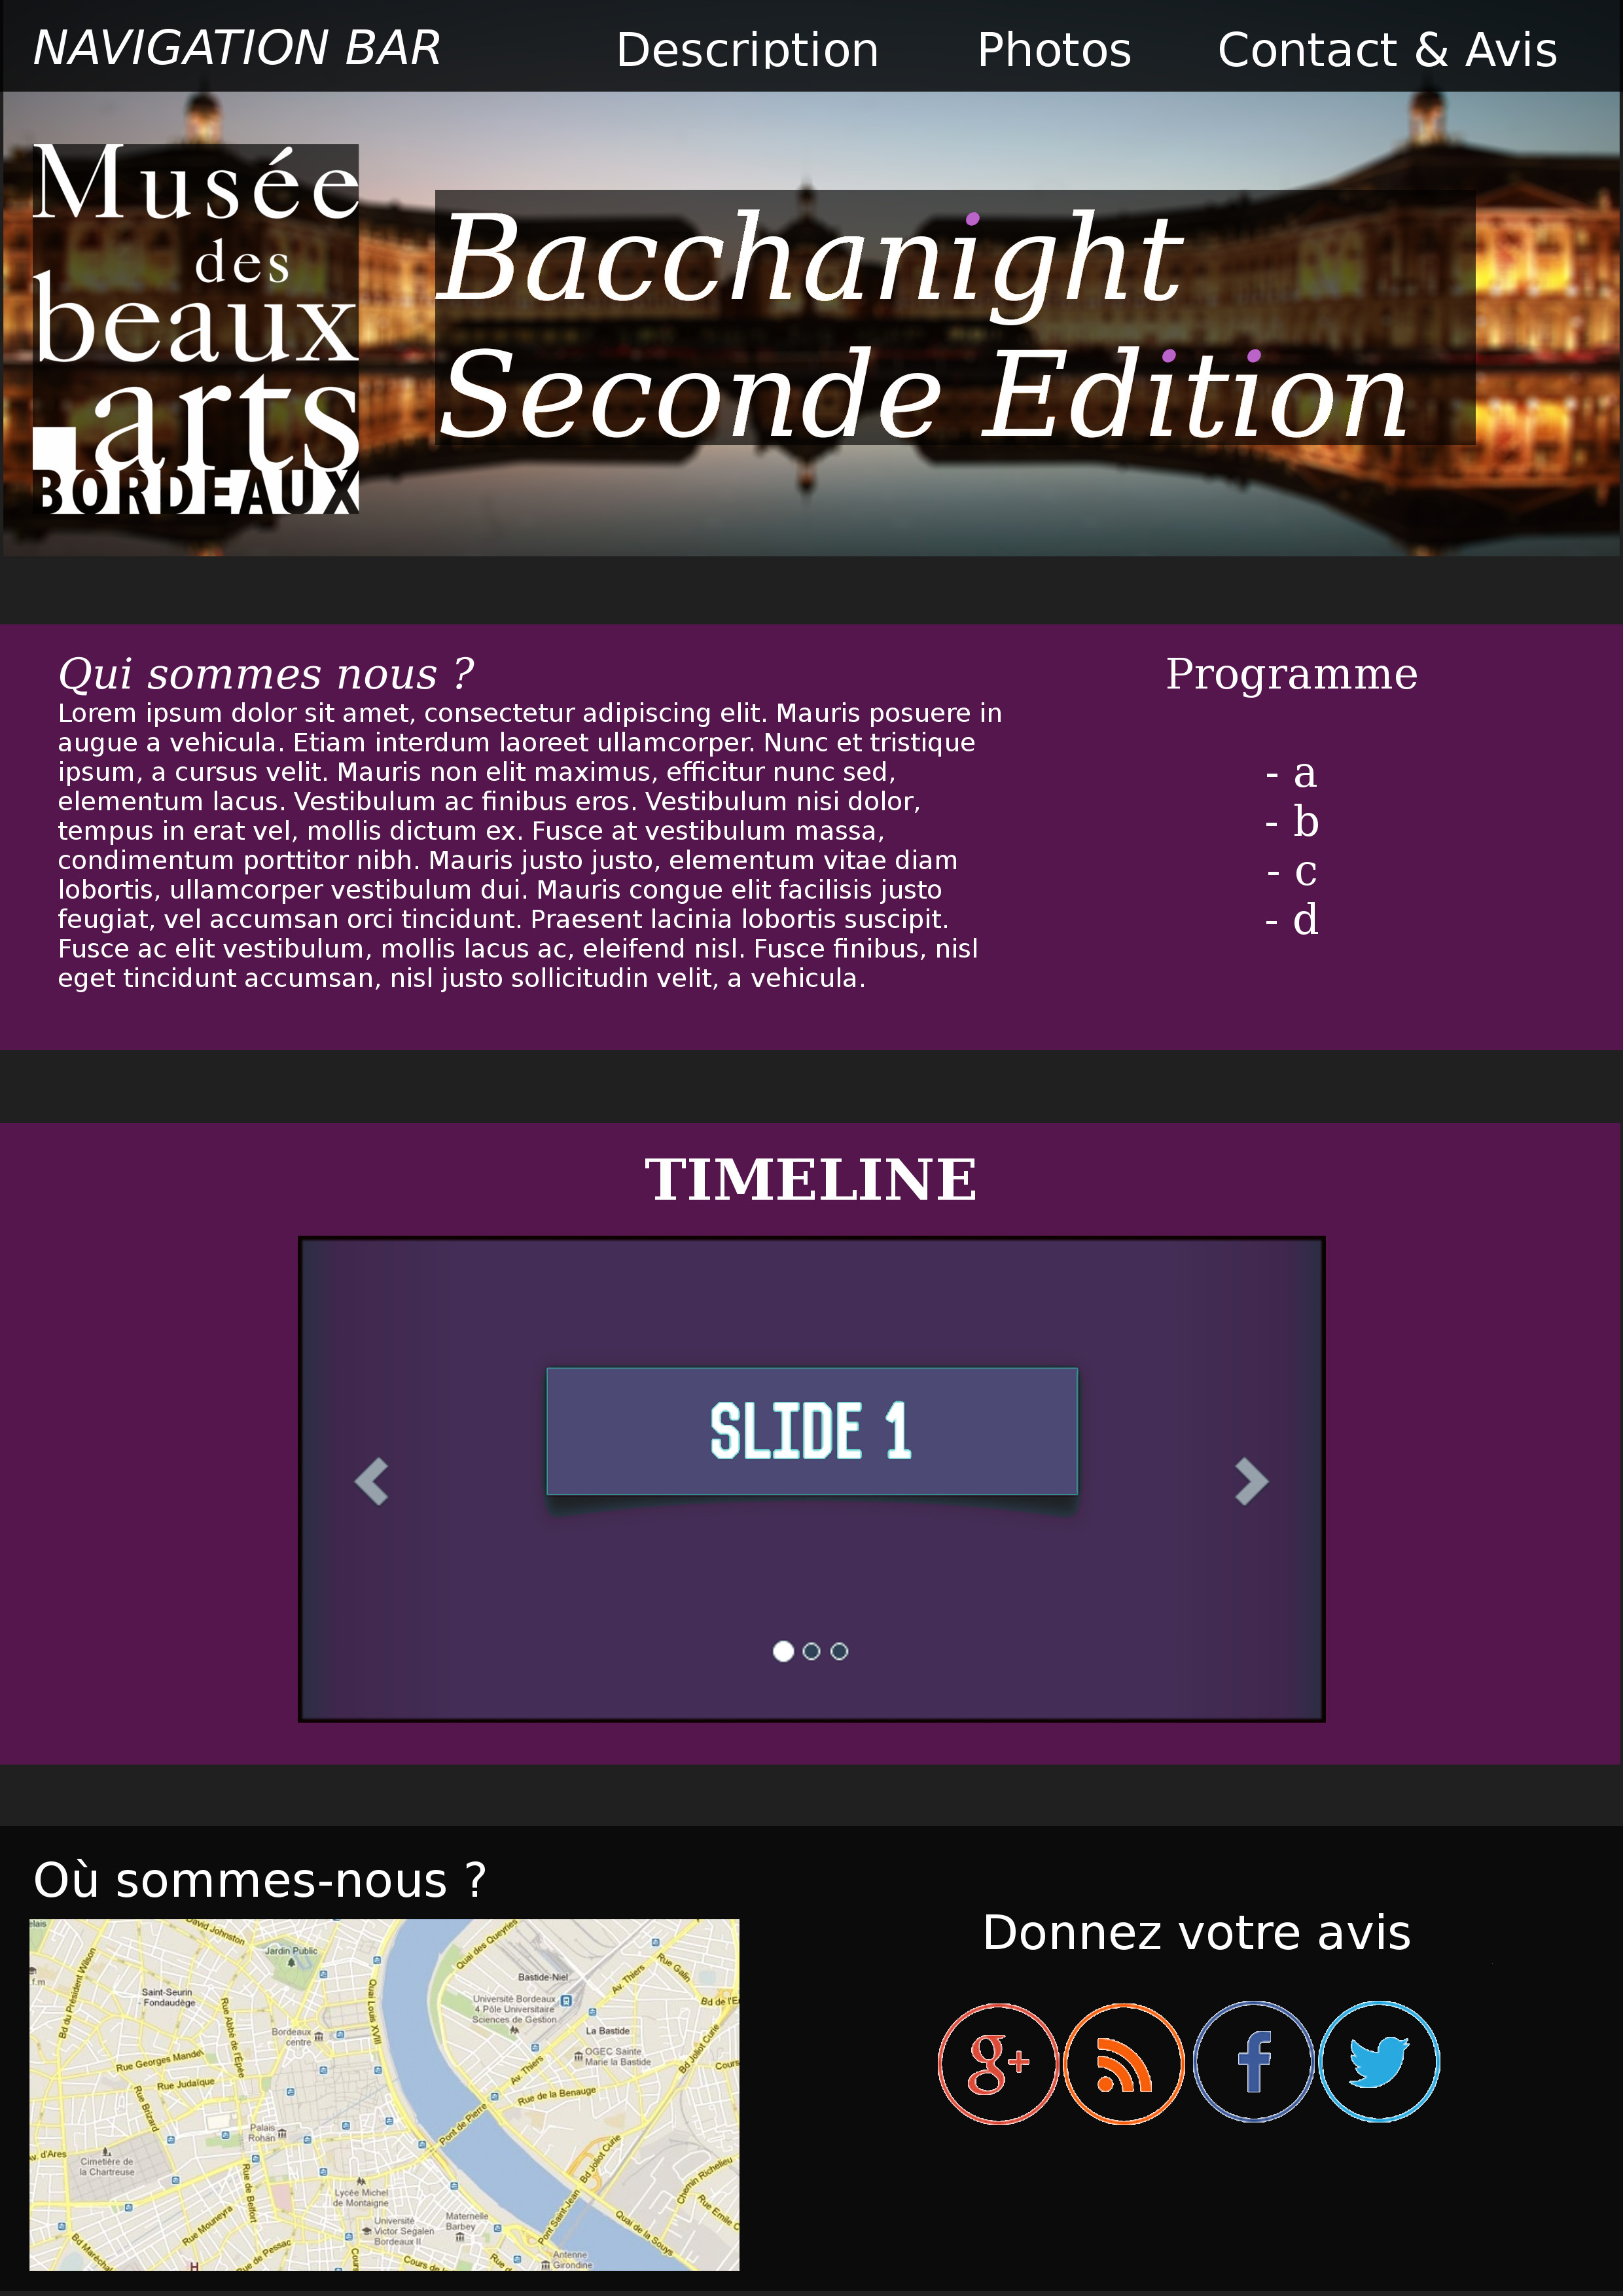
\includegraphics[scale=0.75]{maquette.jpg}

\end{document}
